\chapter{Diseño software}
\label{chap:soft}
\graphicspath{{soft/figs/}{soft/figs/}}

%******************************************************************************************************************************************************

El protocolo de red es una de las piezas fundamentales en el desarrollo de este trabajo. En este apartado se realizará un análisis detallado de las especificaciones del protocolo, su formato de tramas y las máquinas de estados que gobiernan su funcionamiento.

Teniendo definidas las especificaciones, se describirá el proceso de implementación en la plataforma hardware diseñada: Herramientas de compilación y depuración, drivers utilizados y estructura del proyecto. 

Por último, se realizarán pruebas de funcionamiento, con el fin de comprobar que se cumplen las especificaciones establecidas.


\section{Diseño del protocolo}

La idea principal es diseñar un protocolo poco pesado, diseñado especialmente para redes de sensores. Las siguientes características:

\begin{itemize}
	\item Tramas de tamaños variables
	\item Configurable
	\item Extensible a diferentes arquitecturas de red
	\item Bidireccional 
	\item Debe funcionar sin hardware específico
	\item Fácil utilizar
\end{itemize}

En esta primera versión del protocolo, implementaremos una red con una topología de estrella. Para esto, definiremos dos tipos o comportamientos diferentes para los dispositivos:

\begin{itemize}
	\item \textbf{Nodos:} Son los dispositivos que contienen los sensores. Se conectan a la red administrada por un master. 
	\item \textbf{Master:} Se encargan de administrar los nodos de la red y de redirigir los datos que le llegan a un servidor o base de datos.
\end{itemize}

Como se verá durante el desarrollo, muchos de los formatos de tramas y características utilizados, están inspirados en otros protocolos como el de ethernet y el de LoRaWAN.  

\subsection{Formato de trama}

La trama enviada por el sistema está compuesta por una cabecera de 7 bytes seguida de un payload de tamaño variable entre 1 y 256 bytes. El tamaño de la carga estará limitado por la configuración de sistema.

La representación gráfica de la trama es la siguiente:
\begin{figure}[!h]
	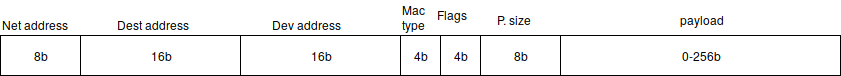
\includegraphics[scale=0.5]{trama.png}
	\centering
	
\end{figure}
\begin{enumerate}
	\item \textbf{Net address } (8b) Identificador de la red en la que se llevan acabo las transacciones. Puede tomar valores entr 0 y 254, el valor 255 está reservado para transacciones broadcast.
	\item \textbf{Dest address } (16b) Identificador del nodo/master destino. 
	\item \textbf{Dev address } (16b) Identificador del nodo/master que realiza la transacción. Este valor puede estar definido por defecto o ser asignada por defecto por un master.
	\item \textbf{Mac type } (4b) Identificado del tipo de trama que se envía. Este puede ser:
	\begin{center}
		\begin{tabular}{|c c c|}
			\hline
			Tipo & Identificador & Descripción \\
			\hline \hline
			TX   & 0 & Trama de datos \\
			JOIN & 3 & Trama de conexión \\
			ACK  & 1 & Trama de asentimiento \\
			NACK & 2 & Trama de Asentimiento negativo \\
			\hline 
	\end{tabular}
	\end{center}
	\item \textbf{Flags } (4b) Flags de la trama. aún no usadas.
	\item \textbf{P. Size } (8b) Tamaño de la carga de la trama (expresado en bytes)
	\item \textbf{Payload } (0-254) Carga de la trama. Los datos que contenga depenederán del tipo de trama (Mac type). 
	
	\end{enumerate}


\subsubsection{Trama de conexión} \label{ConnectionPay}

	Al iniciarse un nodo, este intentará conectarse a una red (conocida o cercana). Para  hacerlo, enviará un paquete cuyo payload contendrá el identificador único de nodo así como el formato de trama que utilizará en la transacción. El formato es el siguiente:
	
	\begin{figure}[!h]
		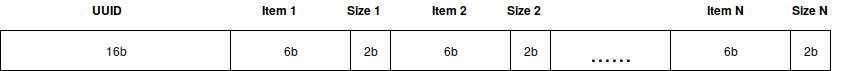
\includegraphics[scale=0.5]{trama_join.png}
		\centering
	\end{figure}

	\begin{enumerate}
		\item \textbf{UUID } (16b) Identificador único del nodo.
	 	\item \textbf{Item N} (6b) Identificador del tipo de dato a enviar. puede ser:
		
		\begin{center}
			\begin{tabular}{|l c l|}
				\hline
				Tipo & Identificador & descripción \\
				\hline \hline
				LIGTH 		& 0x0 & sensor lumínico \\
				PRESURE 	& 0x1 & Sensor de presión \\
				HUMIDITY 	& 0x2 & sensor de humedad \\
				TEMPERATURE	& 0x3 & Sensor de temperatura \\
				.			& . & . \\
				.			& . & . \\
				.			& . & . \\
				CUSTOM 1	& 0x3C & Uso personalizado \\
				CUSTOM 2	& 0x3D & Uso personalizado \\
				CUSTOM 3	& 0x3E & Uso personalizado \\
				\hline
			
			\end{tabular}
		\end{center}
	
		\item \textbf{Size N} Identifica el tamaño del \textbf{Item}. puede tomar los siguientes valores:
		
		\begin{center}
			\begin{tabular}{|c c|}
			\hline
			Identificador & Tamaño \\
			\hline \hline
			0x0	&	1b \\
			0x1 &	8b \\
			0x2	&	16b \\
			0x3 &	24b\\
			\hline
			\end{tabular}
		\end{center}
	\end{enumerate}
	
\subsubsection{Trama de configuración} \label{ConfigPay}
	
	
	Cuando es enviada por un master, contiene la configuración que deberá utilizar el nodo. El formato de trama es el siguiente:
	
	\begin{figure}[!h]
		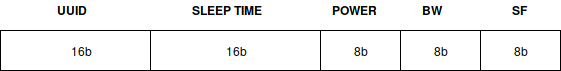
\includegraphics[scale=0.5]{payload_config.png}
		\centering
	\end{figure}
	
	\begin{enumerate}
		\item \textbf{UUID } (16b)Identificador único del nodo (este no cambia, solo se utiliza en la verificación)
		\item \textbf{SLEEP TIME } (16b) Tiempo entre transacciones (segundos). durante ese tiempo el nodo estará dormido
		\item \textbf{POWER } (8b) Potencia de salida de trasmisión (menor o igual a XdBm)
		\item \textbf{BW } (4b) Identificador del ancho de banda del canal. Pude tomar los valoes:
		\begin{center}
			\begin{tabular}{| c c |}
				\hline
				Identificador & Ancho de banda (KHz) \\
				\hline \hline
				0x1 & 125\\
				0x2 & 250 \\
				0x3 & 500 \\
				\hline
		
			\end{tabular}
		\end{center}

		\item \textbf{SF} (4b) Identificador del spreading factor* del transmisor. Puede tomar los valores:
		\begin{center}
			\begin{tabular}{|c c|}
				\hline
				Identificador & SF \\
				\hline \hline
				0x1 & SF7 \\
				0X2 & SF8 \\
				0x3 & SF9 \\
				0X4 & SF10 \\
				0x5 & SF11 \\
				0X6 & SF12 \\
				\hline
			\end{tabular}
		\end{center}
		
		\item \textbf{RXW} (8b) valor de la ventana de recepción (en segundos).
	\end{enumerate}
	

\subsubsection{Trama de datos}

	
	Los datos tendrán el orden y el tamaño definido en la primera conexión. Se puede expresar mediante el siguiente esquema:
	
	\begin{figure}[!h]
		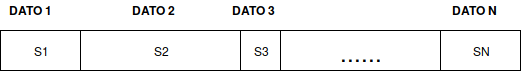
\includegraphics[scale=0.5]{payload_data.png}
		\centering
	\end{figure}
	
\subsection{Comportamiento del protocolo}
 En este apartado se definirá el comportamiento del sistema ante diferentes eventos. Entre ellos podemos encontrar:
	\subsubsection{Conexión de un nodo a la red}
	
	Cuando un nodo pretenda conectarse a un red, enviará una trama de conexión con la información referente a los sensores que tiene implementados y el tamaño del dato. Este paquete se puede enviar en modo broadcast (si se desconoce la red a la que se pretende conectar) o especificando una dirección de red. 
	
	El master, al recibir una trama de conexión, responderá con una trama de configuración con los parámetros que usará el nodo durante su funcionamiento. El funcionamiento se puede resumir en el siguiente cronograma:
	
	\begin{figure}[!h]
		\centering
		%\includegraphics[width = \linewidth]{}
		\caption{Cronograma de conexión de un nodo}
		\label{fig:crono}
	\end{figure}
	
	
	\subsubsection{Envío y recepción de datos}
	
	Estando el nodo conectado a la red, podrá enviar datos al master siguiendo el formato de datos especificado en el proceso de conexión. El nodo podrá enviar tramas con una separación temporal mínima entre ellas. El tiempo de espera entre tramas la especifica el master en la trama de configuración (valor de \textit{Sleep Time}).
	
	Tras enviar un dato, el nodo abrirá un ventana de recepción, cuya duración se especifica en la trama de configuración (valor de \textit{RXW}). Durante ese tiempo, estará a la espera de datos del master. Existe la opción de hacer transacciones con asentimiento (ACK o NACK), pero   no es recomendable en redes con muchos sensores debido a las limitaciones de uso del canal.
	
	
	
	\subsubsection{Tratamiento de errores} \label{ErrorHandle}
	
	El sistema deberá se robusto frente a errores. La forma en la que el sistema responderá a erroes será la siguiente:
	
	\begin{table}[!h]
			\begin{tabularx}{\textwidth}{|X|X|X|}
    			\hline
    	Nombre & descripción & solución \\
    	\hline \hline
    	
    	RX\_ERROR & Paquete recibido dañado o con formato desconocido  & Se incrementará el contador de errores. 
    	Nodo: Si se supera el numero de máximo de errores volverá al proceso de JOIN. Master: descarta el paquete  \\ \hline
    	RX\_NACK  & El nodo master ha recibido un paquete dañado o con formato desconocido &  Se incrementará el contador de errores. Si se supera el numero de máximo de errores volverá al proceso de JOIN \\ \hline
    	TX\_TIMEOUT & Se ha superado el tiempo máximo para enviar un paquete &  Se reconfigura la radio. \\ \hline
    	RX\_TIMEOUT & Se ha superado el tiempo máximo para recibir un paquete &  Si el sistema está configurado para recibir ACK, el sistema pasará a dormir un tiempo aleatorio antes de intentar enviar un nuevo paquete \\ \hline
    	CONF\_ERROR & Existe un error el el paquete de configuración & Se carga la configuración inicial en el nodo y vuelve a start \\ \hline
    	
    	      PR\_ERROR & Error al procesar la trama: Formato desconocido o datos incoherentes & Se descarta la trama y se carga un mensaje tipo NACK en el buffer de salida \\
         \hline
    	\end{tabularx}
    	
	\end{table}
	
	\section{Implementación}
	
	\subsection{Fundamentos teóricos}
		\subsubsection{Sistemas embebidos}
		
		Un sistema embebido es un sistema, que a diferencia de los sistemas de propócito general, está diseñado para realizar unas pocas funciones específicas. Estas funciones, generalmente, tienen requisitos de ejecución de tiempo real.
		
		Estos sitemas suelen tener recursos limitados y requisitos  estrictos. Por este motivo, existe un gran compromiso entre el hardware y el software (la manipulación del hardware se hace de forma directa), lo que limita su programación a lenguajes de bajo nivel.
		
		En la mayoría de los casos, estos sistemas no pueden tener intervención humana, por lo que sus principales características deben ser:
		
		\begin{itemize}
			\item \textbf{Fiabilidad: }El sistema debe tener una tasa de fallos baja.
			\item \textbf{Robustez frente a fallo: }En caso de fallo, el sistema debe ser capaz de recuperarse de manera eficiente.
			
			\item \textbf{Disponibilidad: }El sistema debe estar disponible en el menor tiempo posible.
			
			\item \textbf{Seguridad: }En muchos caso, deben contar con funciones y protocolos que aseguren la integridad de los datos y eviten su acceso a terceros.
		\end{itemize}
		
		
		
		\subsubsection{Sistemas operativos de tiempo real (RTOs}
		Un sistema operativo de tiempo real (también conocido como RTOs por sus siglas en inglés), es un sistema operativo ligero, diseñado para sistemás embebidos con requisitos temporales estrictos. Los RTOs permite la ejecución de código organizado en forma de tareas independientes y gerarquizadas.
		
		Un RTO se puede describir como un "planificador de tiempo real", ya que su función principal es organizar tareas según su prioridad y ejecutarlas garantizado tiempos de ejecución. También, administran los accesos a memoria y los recursos compartidos mediante la implemetación de mutex, semáforos, colas, etc. Estos sistemas son especialmente útiles en microcontroladores con un único núclero, los cuales solo pueden ejecutar una taréa de manera simultanea.
		
		La utilización de un RTOs tiene grandes ventajas que facilitan el desarrollo, depuración y mejora de un sistema, entre ellas podemos encontrar:
		
		\begin{itemize}
			\item \textbf{Abstracción del manejo del tiempo: }Un sistema operativo de tiempo contiene las herramientas necesarias para controlar los tiempo de ejecución. 
			\item \textbf{Escalabilidad y modularidad: }La organización del código en forma de tareas independientes, permite añadir, quitar o modificar módulos de manera rápida y sin comprometer el funcionamiento global del sistema.
			\item \textbf{Reutilización del código: }La utilización de tareas independientes, también permite migrar módulos a otros proyectos.
			
			\item \textbf{Control del consumo: }Los RTOs permiten tener un control estricto de los tiempo de ejecición, lo que se traduce en un mejor control del consumo del sistema.
			
			\item \textbf{Fácil depuración: }Las tareás independientes pueden ser depuradas de forma individual y aislada.
			
			 
		\end{itemize}
		
				
		\subsubsection{Máquinas de estados extendidas (xFSM)}
		
		
		
		\subsubsection{Colas circulares }
		
	\subsection{Descripción del entorno}
		\subsubsection{Drivers, Librerías y útiles}
			Para la implementación del sistema, se han utilizado diferentes drivers para facilitar el proceso de implementación. Estos drivers son los encargados de controlar y gestionar los diferentes periféricos del microcontrolador y el transceptor de LoRa. Los drivers utilizados han sido diseñados por STM y Semtech para sus dispositivos, entre ellos encontramos:
			
			\begin{itemize}
				\item \textbf{HAL drivers:}  la \textit{Hardware Abstraction Layer} es una iniciativa de STMicroelectronics creada con el fin de reducir el tiempo y dificultad de desarrollo de sistemas. Está compuesta por un conjunto de APIs (\textit{Aplication Programin Interfaces} por sus siglas en inglés) que permiten inicializar, configurar y manipular los diferentes periferícos de los microcontroladores de STM. Estos drivers están accesibles a  través de la red bajo una licencia de software libre BSD.
				
				\item \textbf{LoRa drivers:} Diseñados por Semtech, permiten y control de sus tranceptores de LoRa. Son accesibles a través de la red y, al igual que los drivers de STM, están bajo una licencia BSD.
			\end{itemize}			 
			
			Como base para el proyecto, se ha utilizado uno de los ejemplos elaborados por STM para su placa de desarrollo "B-L072Z-LRWAN1", la cual se ha utilizado durante el proceso de implementación. Para utilizar este ejemplo, ha sido necesario modificar el driver de tranceptor, así como las secciones de configuración del hardware. La finalidad de las modificaciones era eliminar las dependencias internas con el middleware de LoRaWAN, el cual se encontraba implementado por defecto. También se modificó la estructura del proyecto y el sistema de compilación.
			\paragraph{}
			
			A parte de estas herramientas, también se han utilizado otras herramientas provenientes de terceros, para la implementación de las máquinas de estados y para el sistema operativo de tiempo real. Las herramientas son:
			
			\begin{itemize}
				\item \textbf{FreeRTOs: } Es una implementación del kernel de un sistema operativo de tiempo real, diseñado para sistemas embebidos. Su uso de ha popularizado por la cantidad de plataformas con la que es compatible, lo bien documentado que está y por estar bajo una licencia de software libre MIT. 
				\item \textbf{FSM: } Es una implementación de una maquina de estados, realizada por ----- e inspirada en la maquina propuesta por ----. Es una implementación sencilla y fácilmente escalable.
			\end{itemize}

				
				El middleware de FreeRTOs ha sido implementado utilizando la configuración propuesta por STM para su microcontrolador. Por otro lado, la implementación del FSM ha sido modificada para comprobar bits de estado y no funciones en las transiciones de estados.
			
		\subsubsection{Herramientas de edición, compilación y depuración} \label{soft:debugApp}
		
		El software de este TFG se ha desarrollado completamente sobre un sistema operativo linux pero, procurando su compatibilidad con otros sistemas operativos. Para ello, se han utilizado herramientas software libres y multiplataforma.
	\paragraph{}
	Para configurar el proyecto se ha utilizado \textit{Cmake}. Cmake es una herramienta libre y multiplataforma diseñada para compilar y probar software. Esta herramienta permite generar ficheros de configuración con independencia del sistema operativo y el compilador utilizado. 
	\paragraph{}
	Como compilador se ha utilizado el conjunto de herramientas \textit{GCC ARM Embedded}. GCC ( GNU Compiler Collection por sus siglas en inglés), es un conjunto de compiladores y librerías, creados por el proyecto GNU, que permiten la compilación de código en C, C++, Ada y Fortran. Concretamente, se ha utilizado la variante para arquitecturas ARM, la cual permite la compilación cruzada del código.
	\paragraph{}
	Para depurar el código, se han utilizado las herramientas GDB y STLINK. STLINK es un circuito integrado que permite la depuración y programación de microcontroladores STM32. Por otro lado, GDB (GNU Debugger) es un depurador de lenguajes como C y C++ que permite ejecutar instrucción a instrucción el programa y conocer, en cada momento, el estado de los registros y memoria. 
	
				
	\subsection{Modelado del comportamiento de los nodos} \label{NodeFSM}
	
	\begin{figure}[!h]
		\centering
		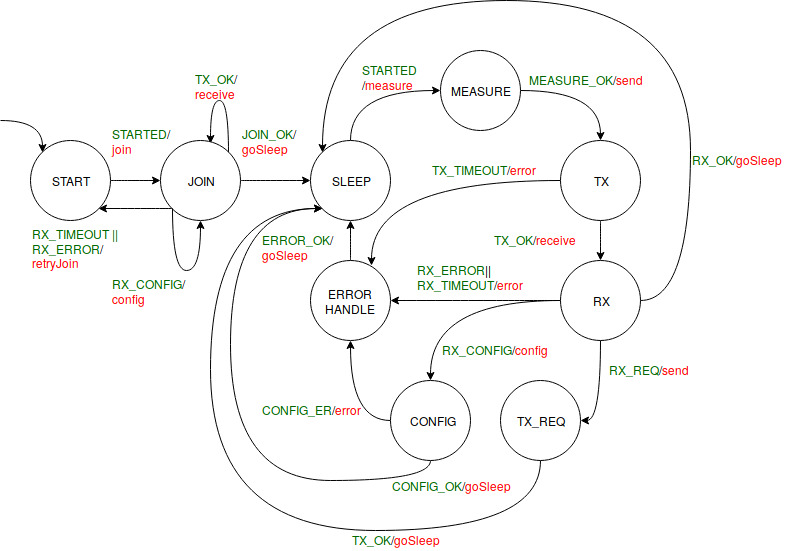
\includegraphics[width=0.75\linewidth]{FSM_NODE.jpg}
		\caption{Esquema de modelado de los nodos mediante máquinas de estado}
		\label{fig:nodeFSM}
	\end{figure}
	
	El sistema se ha modualdo mediante máquinas de estado extendidad cuyo comportamiento de los nodos se puede ver resumido en la figura \ref{fig:nodeFSM}. La función principal de los nodos será enviar datos referentes a los sensores de forma periódica al nodo maestro. 
	El comportamiento del nodo cuenta con los siguientes 8 estados:
	
	\begin{itemize}
		\item \textbf{JOIN:} Los nodos intentarán establecer una conexión con un master. Para ello, enviaran un paquete de tipo JOIN como el especificado en la sección \ref{ConnectionPay}. Al llegar un paquete con estas características, el master responderá con un paquete tipo CONFIG con la configuración del nodo, siguiendo el formato visto en la sección \ref{ConfigPay} . Si el paquete de configuración contiene información válida, el sistema iniciará su funcionamiento habitual. El sistema solo volverá a JOIN si se reinicia ó, si la función esta habilitada, si supera el número máximo de paquetes tipo NACK definido.
		
		\item \textbf{SLEEP: } El sistema entrará en bajo consumo durante el tiempo definido. En este estado, se deshabilitaran los recursos no esenciales con el fin de minimizar el consumo del sistema.
		
		\item \textbf{MEASURE: } El sistema procesará las entradas de los sensores y cargará los datos en el buffer de salida. El formato de trama tendrá que coincidir con el especificado en proceso de JOIN, de lo contrario el nodo master responderá con un mensaje tipo NACK.
		
		\item \textbf{TX: } El sistema enviará los elementos del buffer de salida. En caso de error, este será tratado.
		
		\item \textbf{RX: } Tras enviar los datos, se abrirá una ventana de recepción a la espera de un paquete de datos. En caso de error, este será tratado.
		
		\item \textbf{CONFIG: } Si el el paquete recibido es de tipo configuración (ver sección \ref{ConfigPay}), esta se cargará en el sistema y será utilizada en la siguiente transacción.
		
		\item \textbf{TX\_REQ: } Si el paquete recibido es del tipo request info, se cargará la información del sistema en un paquete tipo configuración y se enviará al nodo master. (TODO -> revisar)
		
		\item \textbf{ERROR\_HANDLE: } Si ocurriese algún error durante la ejecución de alguno de los procesos, este se capturara y se intentará buscarle
una solución. La forma en la que se tratarán los erroes, se encuentra especificada en la sección \ref{ErrorHandle}.
		
		
	\end{itemize}
	
	\subsection{Modelado del comportamiento del nodo maestro}
	
	\begin{figure}[!h]
		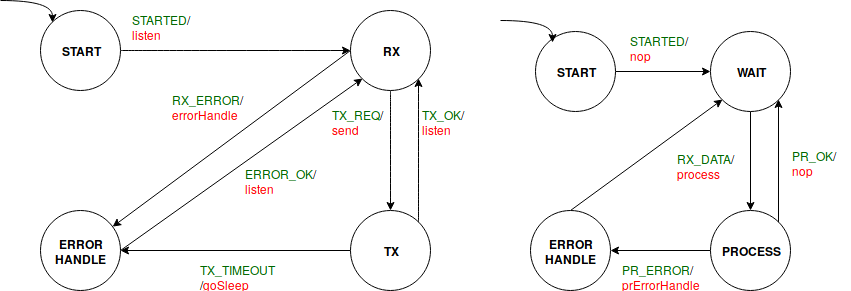
\includegraphics[width=\linewidth]{FSM_MASTER.png}
		\caption{Modelado del comportamiento mediantes maquinas de estado extendidas}
		
		\label{fig:MasterFSM}
	\end{figure}
	
	A diferencia de los nodos vistos en el apartadado \ref{NodeFSM}, el comportamiento de los nodos maestros se ha modelado mediante dos máquinas de estados. La principal motivación de este cambio, será separar la funciones de recepción y transmisión de paquetes de las funciones de procesado de datos, de esta forma, evitamos la perdida de datos durante procedentes de los nodos. Todo esto es posible gracias a las posibilidades que nos ofrecese FreeRTOs y las máquinas de estados extendidas.
	
	los estados de la máquina de recepción de datos son los siguientes:
	
	\begin{itemize}
		\item \textbf{RX: }Este es el estado por defecto del receptor. Se encuentra siempre escuchando el canal a la espera de datos. Cuando recibe datos los encola en una cola circular y avisa a la segunda máquina de la prescencia de datos.
		\item \textbf{TX: }Cuando la segunda máquina notifica la existencia de datos en el buffer de salida, esta envía los datos y vuelve a su estado por defecto.
		\item \textbf{ERROR\_HANDLE: } Recupera al sistema de los errores notificados por otros estados.
	\end{itemize}
	
	Por otro lado, los estados asociados al procesado de datos son los siguientes:
	
	\begin{itemize}
		\item \textbf{WAIT: }Se matiene a la espera de datos.
		\item \textbf{PROCESS: }Cuando existen datos encolados, los procesa y genera un respuesta.
		\item \textbf{ERROR\_HANDLE: }Recupera el sistema de un error.
	\end{itemize}
	
	Los estados y las transiciones asociadas de cada máquina se pueden ver resumidos en la figura \ref{fig:MasterFSM}.
	
	\subsection{Estructura del código}
	\subsection{Proceso de diseño e implementación}
	\subsection{Resultados obtenidos}
	
	
	